\subsection{単一気泡上昇：浮力残差と projection の共有}
\label{sec:val_rising_bubble}
% ═══════════════════════════════════════════════════════════════════

\subsubsection{設定と理論的焦点}

単一気泡上昇ベンチマークでは，水中に空気円を置き，
実重力下で上昇させる．
幾何は Hysing 型の単一気泡配置~\cite{Hysing2009}を参照するが，
物性と長さは $10\,\mathrm{mm}$ 級の水--空気系へ戻し，
目的を「終端速度表の再現」だけに置かない．
本ケースの焦点は，表面張力の pressure-jump 閉包と，
浮力分解
\[
  \rho\bm{g}=-\bnabla(\rho\Phi_g)+\Phi_g\bnabla\rho
\]
から得る face residual acceleration が，同じ projection 空間で閉じるかにある．
hydrostatic な勾配成分を nodal predictor に直接入れると，
projection で消えるべき力が非ソレノイダル速度として残る．
したがって浮力残差は，PPE と同じ $A_f,G_f,D_f$ 上で評価する．

\begin{itemize}[noitemsep,leftmargin=2em]
  \item グリッド：$[0,0.01]\times[0,0.02]\,\mathrm{m}$，
        $32\times64$，$x$ 周期/$y$ 壁面，static interface-fitted $\alpha=2$
  \item 初期界面：中心 $(0.005,0.005)\,\mathrm{m}$，
        半径 $R=0.0025\,\mathrm{m}$ の気泡
  \item 物性：$\rho_l=1000$，$\rho_g=1.2$，
        $\mu_l=10^{-3}$，$\mu_g=1.8\times10^{-5}$，
        $\sigma=0.072$，$g=9.81$
  \item 時間：掲載窓 $0\le t\le0.03\,\mathrm{s}$，
        snapshot は $0.005\,\mathrm{s}$ 刻み，理論 CFL multiplier $1.0$
  \item 出力：\texttt{bubble\_centroid}，
        \texttt{mean\_rise\_velocity}，\texttt{deformation}，
        \texttt{volume\_conservation}，$\psi$/速度/圧力 snapshot
\end{itemize}

\subsubsection{結果と判定}

図~\ref{fig:ch14_rising_bubble_initial_snapshots}に，
現在の論文に掲載する初期窓の $\psi$ snapshot を示す．
$t=0.0299956\,\mathrm{s}$ では，重心は
$y_c=7.350\times10^{-3}\,\mathrm{m}$，
平均上昇速度は $9.57\times10^{-2}\,\mathrm{m/s}$，
変形量は $D=0.343$ であり，
diffuse phase-volume drift は $8.99\times10^{-6}$ に留まる．
したがって $0\le t\le0.03\,\mathrm{s}$ の範囲では，
相体積の漏れではなく，浮力残差と粘性抵抗・表面張力閉包の釣合いとして
初期上昇と変形を読むことができる．

\begin{figure}[!htbp]
\centering
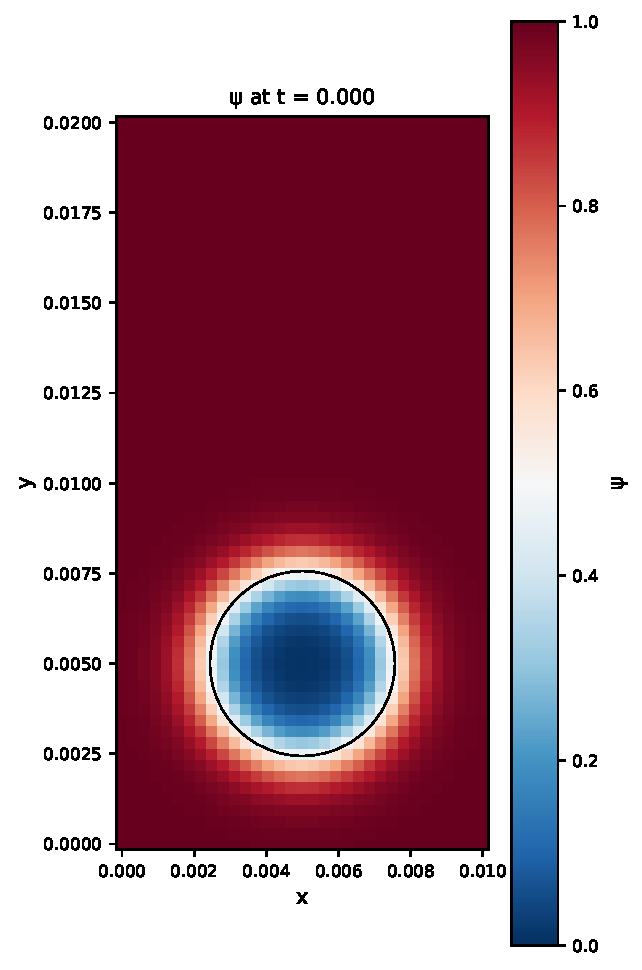
\includegraphics[width=0.23\linewidth]{figures/ch14_rising_bubble_psi_t000.pdf}
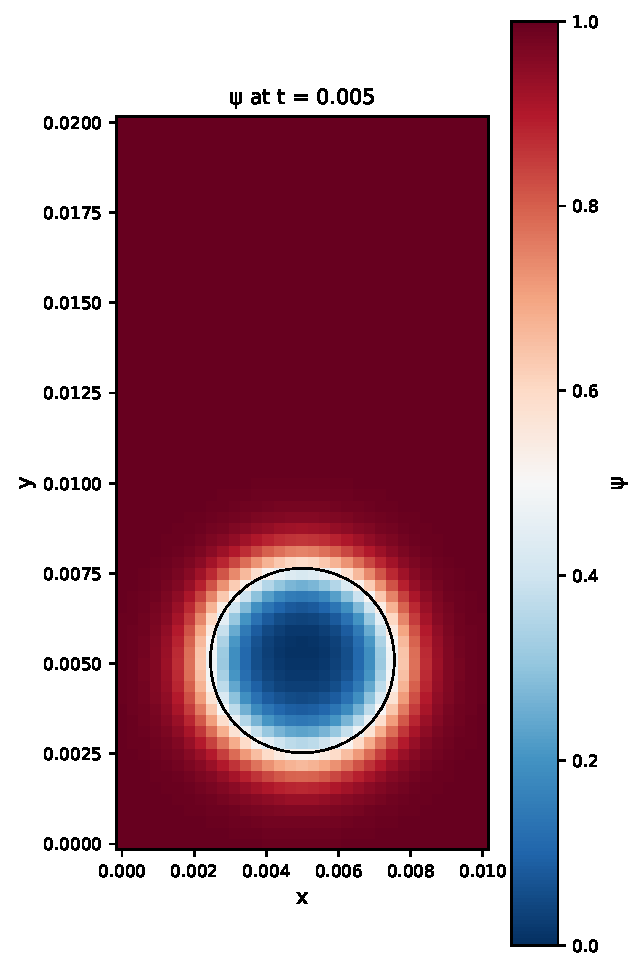
\includegraphics[width=0.23\linewidth]{figures/ch14_rising_bubble_psi_t005.pdf}
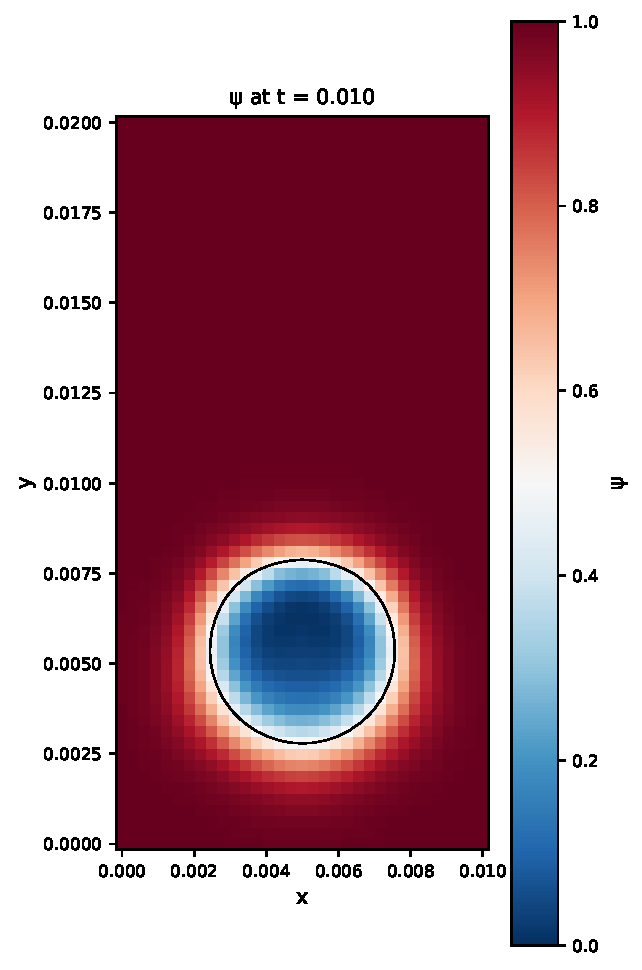
\includegraphics[width=0.23\linewidth]{figures/ch14_rising_bubble_psi_t010.pdf}
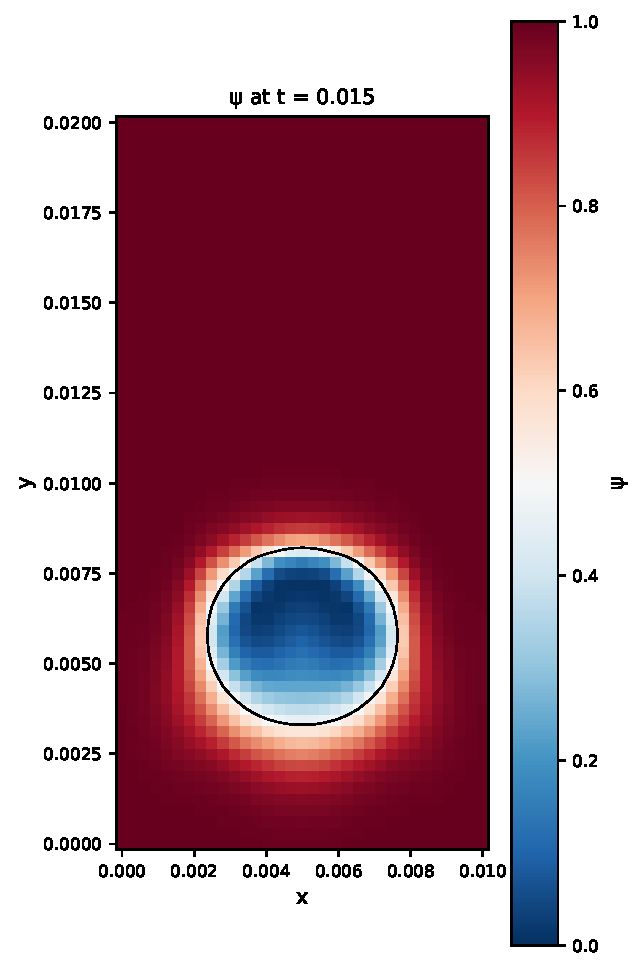
\includegraphics[width=0.23\linewidth]{figures/ch14_rising_bubble_psi_t015.pdf}\\[-0.2em]
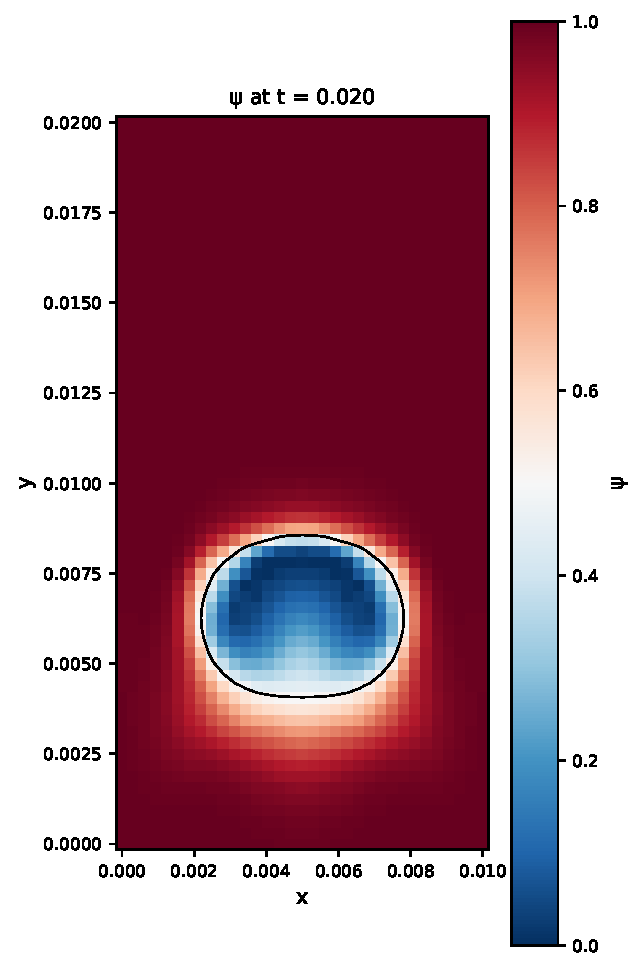
\includegraphics[width=0.23\linewidth]{figures/ch14_rising_bubble_psi_t020.pdf}
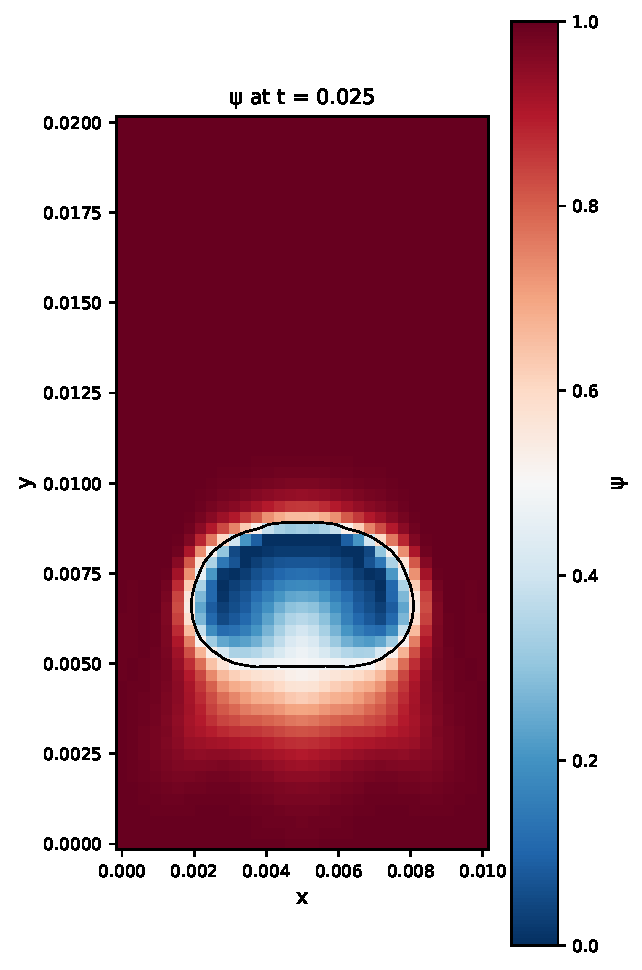
\includegraphics[width=0.23\linewidth]{figures/ch14_rising_bubble_psi_t025.pdf}
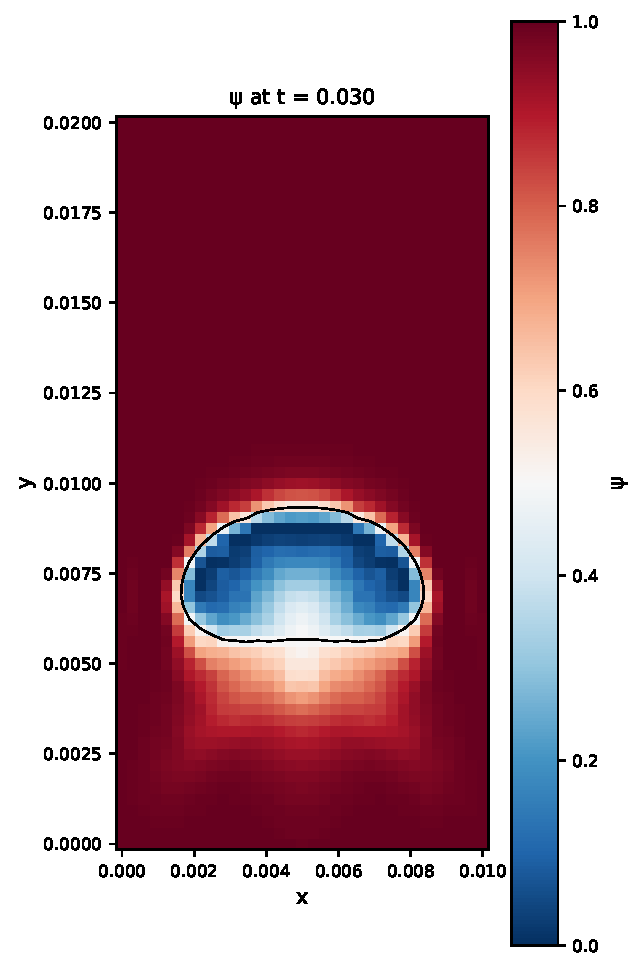
\includegraphics[width=0.23\linewidth]{figures/ch14_rising_bubble_psi_t030.pdf}
\caption{単一気泡上昇の掲載 snapshot．
左上から $t=0,0.005,\ldots,0.03\,\mathrm{s}$ の $\psi$ 場を示す．
本稿では形状破綻が顕在化する前の初期窓だけを掲載対象とする．}
\label{fig:ch14_rising_bubble_initial_snapshots}
\end{figure}

一方，継続計算では $t\simeq0.04\,\mathrm{s}$ 以降に
下側界面の停滞と $\psi=0.5$ 形状の分裂が見え始める．
この破れは，diffuse phase-volume diagnostic が小さいままでも
sharp gas geometry と連結性が保存されないという，
保存すべき不変量の取り違えを示している．
したがって長時間の気泡形状・終端速度ベンチマークとしては採用せず，
幾何 cell-fraction state space で
material volume と gauge profile の互換性を同一 cochain に戻す課題として扱う．

本ケースの判定は，
「$0\le t\le0.03\,\mathrm{s}$ の初期窓では
surface-tension pressure-jump と hydrostatic-balanced buoyancy が
同じ面速度空間の射影に入り，上昇応答を作る．
ただし $t\simeq0.04\,\mathrm{s}$ 以降の形状保存は未解決であり，
本章の合格 claim には含めない」
である．

% ═══════════════════════════════════════════════════════════════════
